\section{Characteristics and Challenges of Microservices}
\label{chap:microservices}
The essential characteristic of a microservice architecture is to develop an business process as a set of small and independent services. These run within their own process and are developed and deployed independently. Figure \ref{fig:microservice} illustrates the granularity of the microservice layer, where the business logic is designed to be very atomic. Each microservice should ideally have its focus on business logic \cite[p. 7]{sm3}.

\begin{figure}
    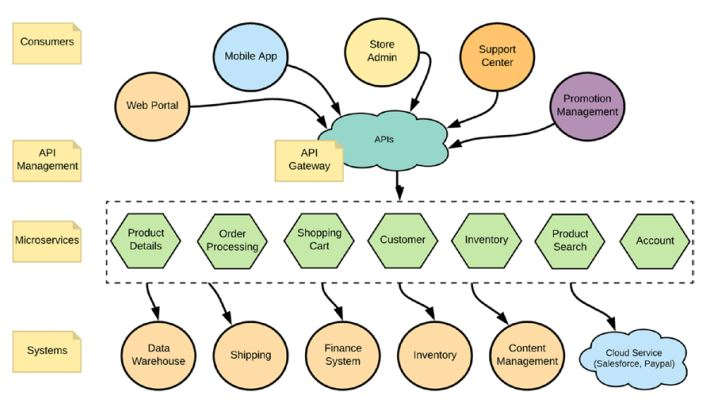
\includegraphics[width=\columnwidth]{img/microservice.JPG}
    \caption{Ex. microservice architecture of an online retail application \cite[p. 7]{sm3}}
    \label{fig:microservice}
\end{figure}

Microservices represent an opposite principle to monolithic architectures. This approach attempts to solve classic problems of a monolithic application, e.g. the deployment. Since all modules in a monolithic application run in one process, the entire application must be redeployed for every change, no matter how small. This is comparatively time-consuming and means that the software is shipped less frequently. Microservices do not have this problem because each service represents a module and is deployed independently. This fact means that teams can develop more independently and new features can be shipped more quickly and frequently \cite{fowler}.

Another key advantage of microservices is that they can be scaled horizontally and independently. A monolith is only vertical scalable by increasing the computing power of the running instance which is limited at some point \cite{fowler}.

Because of the mentioned granularity, the need for interservice communication increases. The complexity of this communication is usually more challenging than the actual business logic implementation. Due to the increased inter-service communication, microservices tend to be more prone to failures. This results in the requirement that a failure of one or more of these services should not bring down the entire application. Therefore, a failure of a microservice should be handled in such a way that it has minimal impact on the business functionalities of the application \cite[p. 11 ff.]{sm3}.

Another important challenge in the microservice context is maintenance. Due to the complexity of the architecture, it is necessary to introduce appropriate tools for e.g. service monitoring \cite[p. 16]{sm3}.